%!TEX TS-program = xelatex
%!TEX encoding = UTF-8 Unicode

\documentclass[a4paper, 12pt]{article}

%\newcommand{\LastChange}{Time-stamp: "2014-07-09 15:59:43 aga SeminarProblems.tex"}


% \usepackage[colorinlistoftodos]{todonotes}
\usepackage[colorlinks=true, allcolors=blue]{hyperref}

%\usepackage{euler}
%\usepackage{xltxtra} % loads: fixltx2e, metalogo, xunicode, fontspec

% \usepackage{multicol} % many columns
\usepackage{amsmath,amsfonts,amssymb,amsthm}
\usepackage{fullpage}
\usepackage{graphicx}
\usepackage{bm}

\usepackage{marvosym} % значок мужского туалета

%\usepackage{enumerate}
\usepackage{textcomp} % text in formulas

%\usepackage{paralist}
\usepackage{enumitem} % more options for lists

\usepackage{tikz} % картинки
\usetikzlibrary{arrows.meta} % tikz-прибамбас для рисовки стрелочек подлиннее

\usepackage[includehead, top=1cm, bottom=1cm, left=1.5cm, right=1.5cm]{geometry}


\usepackage{fontspec} % что-то про шрифты?
\usepackage{polyglossia} % русификация xelatex

\setmainlanguage{russian}
\setotherlanguages{english}

% download "Linux Libertine" fonts:
% http://www.linuxlibertine.org/index.php?id=91&L=1
\setmainfont{Linux Libertine O} % or Helvetica, Arial, Cambria
% why do we need \newfontfamily:
% http://tex.stackexchange.com/questions/91507/
\newfontfamily{\cyrillicfonttt}{Linux Libertine O}

\defaultfontfeatures{Mapping=tex-text}

\AddEnumerateCounter{\asbuk}{\russian@alph}{щ} % для списков с русскими буквами
\setlist[enumerate, 2]{label=\asbuk*),ref=\asbuk*}

%\setmainfont{Times New Roman}
%\setmainfont{Arial}
%\setmainfont{PT Sans}


%\setlength{\topmargin}{0in}
%\setlength{\headheight}{0cm}
%\setlength{\headsep}{0in}
%\setlength{\oddsidemargin}{-0.5in}
%\setlength{\evensidemargin}{-0.5in}
%\setlength{\textwidth}{7.5in}
%\setlength{\textheight}{9.0in}


% \newcommand{\staritem}{\refstepcounter{enumi}\item[\bf *\theenumi.]}

% \newcommand{\bsym}{\boldsymbol}


%\newcommand{\FigWidth}{0.3\columnwidth}



\newtheoremstyle{break}% name
  {}%         Space above, empty = `usual value'
  {9pt}%         Space below
  {}% Body font
  {}%         Indent amount (empty = no indent, \parindent = para indent)
  {\bfseries}% Thm head font
  {.}%        Punctuation after thm head
  {\newline}% Space after thm head: \newline = linebreak
  {}%         Thm head spec

\theoremstyle{break}
\newtheorem{problem}{Задача}[subsection]
\renewcommand{\theproblem}{\arabic{problem}}% Remove subsection from the counter representation


\begin{document}

\thispagestyle{empty}
%%%%%%%%%%%%%%%%%%%%%%%%%%%%%%
%%%%%%%%%%%%%%%%%%%%%%%%%%%%%%
\subsection*{Третий Тур}
%%%%%%%%%%%%%%%%%%%%%%%%%%%%%%

\begin{problem}
Известно, что $a_0 = 3$ и $2a_n - a_{n-1} = 2$. Чему равно $a_{10}$?
\end{problem}

\begin{problem}
Дзюба подбрасывает мяч вертикально с начальной скоростью 12 м/с.
Акинфеев подбрасывает вертикально такой же мяч на секунду позже.
Чему равна начальная скорость мяча Акинфеева,
если он приземлился одновременно с мячом Дзюбы?

Сопротивлением воздуха, а также ростами Дзюбы и Акинфеева можно пренебречь.
Ускорение свободного падения равно $g=10$ м/с$^2$.
\end{problem}



\begin{problem}
Диагонали трапеции равны $d_1$ и $d_2$, а высота к основанию равна $h$. Чему равна площадь трапеции?
\end{problem}



\begin{problem}
Брусок массы $m$ налетает со скоростью $V$ на три неподвижных бруска массами $3m$, $9m$, и $27m$,
расположенных как показано на рисунке. Столкновения абсолютно упругие.
Чему равна скорость бруска массы $27m$ после всех столкновений брусков друг с другом?

Дорогой друг, трением разрешаю тебе пренебречь! Твой главный судья $\heartsuit$.

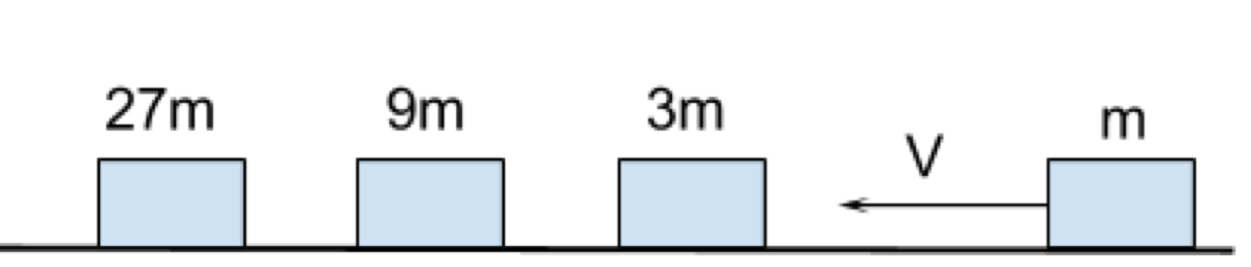
\includegraphics[scale=0.3]{images/m_3m_27m_nowall.png}
\end{problem}




\subsection*{Третий Тур}
%%%%%%%%%%%%%%%%%%%%%%%%%%%%%%
\setcounter{problem}{0}


\begin{problem}
Известно, что $a_0 = 3$ и $2a_n - a_{n-1} = 2$. Чему равно $a_{10}$?
\end{problem}

\begin{problem}
Дзюба подбрасывает мяч вертикально с начальной скоростью 12 м/с.
Акинфеев подбрасывает вертикально такой же мяч на секунду позже.
Чему равна начальная скорость мяча Акинфеева,
если он приземлился одновременно с мячом Дзюбы?

Сопротивлением воздуха, а также ростами Дзюбы и Акинфеева можно пренебречь.
Ускорение свободного падения равно $g=10$ м/с$^2$.
\end{problem}



\begin{problem}
Диагонали трапеции равны $d_1$ и $d_2$, а высота к основанию равна $h$. Чему равна площадь трапеции?
\end{problem}



\begin{problem}
Брусок массы $m$ налетает со скоростью $V$ на три неподвижных бруска массами $3m$, $9m$, и $27m$,
расположенных как показано на рисунке. Столкновения абсолютно упругие.
Чему равна скорость бруска массы $27m$ после всех столкновений брусков друг с другом?

Дорогой друг, трением разрешаю тебе пренебречь! Твой главный судья $\heartsuit$.

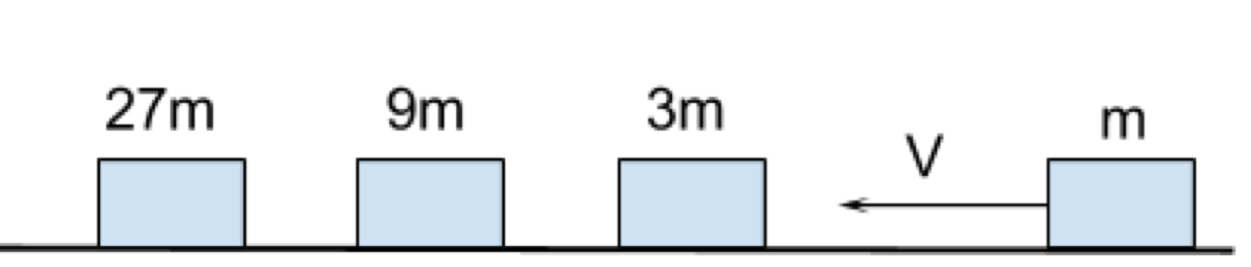
\includegraphics[scale=0.3]{images/m_3m_27m_nowall.png}
\end{problem}



\end{document}
